\documentclass{article}
\usepackage{graphicx}
\usepackage[margin=1.5cm]{geometry}
\usepackage{amsmath}

\begin{document}
\twocolumn

\title{Friday Warm Up: Unit 5: Momentum II}
\author{Prof. Jordan C. Hanson}

\maketitle

\section{Memory Bank}

\begin{itemize}
\item $\vec{p} = m\vec{v}$ ... Definition of momentum.
\item $\vec{p}_{\rm total} = \vec{p}_1 + \vec{p}_2$ ... Total momentum.
\item $\vec{p}_{\rm total,i} = \vec{p}_{\rm total,f}$ ... Momentum is conserved.
\item $\vec{F}_{\rm Net} = \frac{d\vec{p}}{dt}$ ... Force and momentum
\item Let $M$ be the total mass of a system, and let $m_j$ and $\vec{r}_j$ $(j = 1,...,N)$ be the masses and positions of the constituent parts of the system.  The position of the center of mass is
\begin{equation}
\vec{r}_{\rm CM} = \frac{1}{M}\sum_{j=1}^{N}m_j \vec{r}_j
\end{equation}
\item The momentum of the center of mass $\vec{P}_{\rm CM}$ is
\begin{equation}
\vec{P}_{\rm CM} = \sum_{j=1}^N \vec{p}_j
\end{equation}
\item The net external force on a system obeys
\begin{equation}
\vec{F} = \frac{d\vec{P}_{\rm CM}}{dt}
\end{equation}
\end{itemize}

\section{Momentum II}

\begin{enumerate}
\item An alpha particle (4 amu) undergoes an elastic collision with a stationary uranium nucleus (235 amu).  What percent of the kinetic energy of the alpha particle is transferred to the uranium nucleus? Assume the collision is one-dimensional. \\ \vspace{4cm}
\item Three point masses are placed at the corners of a triangle as shown in Fig. \ref{fig:1}.  Find the center of mass of the three-mass system. \\ \vspace{3cm}
\item Two objects of equal mass $m$ approach each other with equal speed $v$.  The undergo a totally inelastic collision.  Determine the location of the center of mass versus time, before and after the collision.
\end{enumerate}

\begin{figure}
\centering
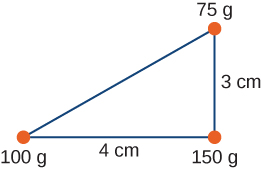
\includegraphics[width=0.25\textwidth]{figures/triangle.jpeg}
\caption{\label{fig:1} Triangle of masses.}
\end{figure}

\end{document}
